% !TEX root = ../licenta.tex
\chapter{Framework and Technology Stack}
\label{ch:framework_tech_stack}

\section{Introduction to the Architectural Paradigm}
The development of a robust, production-grade Time Series Forecasting Visualizer presents a unique intersection of software engineering and econometric challenges. Historically, the domain of time series analysis has been monopolized by procedural, script-based environments---most notably R-Studio, MATLAB, and localized Python kernels (such as Jupyter Notebooks). While these environments excel at executing dense mathematical matrix operations and generating static visualizations historically, they fundamentally lack the infrastructure required to deploy scalable, interactive, and responsive web-based User Interfaces (UIs) accessible to non-technical executive stakeholders. 

Conversely, traditional monolithic web application stacks (such as LAMP—Linux, Apache, MySQL, PHP, or Java Spring Boot architectures) excel at rapid interface rendering and database queries but lack the native, open-source, peer-reviewed mathematical libraries capable of executing complex linear algebra, seasonal decompositions, or Bayesian change-point detections efficiently. 

To bridge this operational and computational divide, the architecture of this application was designed utilizing a highly optimized, native JavaScript paradigm. Rather than relying on clunky cross-language IPC bridges, the system forcefully ports complex econometric math directly into the Node.js V8 execution engine.

\begin{figure}[H]
\centering
\begin{tikzpicture}[node distance=2.5cm]
\node (client) [abstractbox] {React Frontend (Vite)};
\node (express) [processbox, below=of client] {Node.js Express API};
\node (python) [abstractbox, left=of express] {V8 Native Math (PELT)};
\node (gemini) [abstractbox, right=of express] {Google Gemini API};
\node (user) [iobox, above=of client] {Executive Operator};

\draw [arrow] (user) -- node[anchor=west, font=\scriptsize] {CSV Upload} (client);
\draw [arrow] (client) -- node[anchor=west, font=\scriptsize] {JSON Matrix / Axios} (express);
\draw [arrow] (express) -- node[anchor=south, font=\scriptsize] {Native Call} (python);
\draw [arrow] (express) -- node[anchor=south, font=\scriptsize] {HTTPS Payload} (gemini);
\draw [dashedarrow] (python) edge[bend right=40] node[anchor=north, font=\scriptsize] {Computed Array} (express);
\draw [dashedarrow] (gemini) edge[bend left=40] node[anchor=north, font=\scriptsize] {Generated Text} (express);
\draw [dashedarrow] (express) edge[bend right=40] node[anchor=west, font=\scriptsize] {SVG Coordinates} (client);
\end{tikzpicture}
\caption{The Integrated Native System Architecture. The Node.js Server acts as the central orchestrator executing pure mathematical data natively and receiving analytical strings from Generative AI.}
\label{fig:sys_arch}
\end{figure}

The diagram presented in Figure \ref{fig:sys_arch} represents the exact telemetry data takes. By executing the analytical processing natively via V8 algorithms and decoupling the generational synthesis (Google Gemini) logically via external REST calls, the system prevents severe memory blockages without ever paying the computational cost of cross-language latency.

\section{The Frontend Presentation Layer: React.js and TypeScript}

The client-facing frontend represents the user's entire interactive experience with the mathematical engine. The primary requirement for the frontend was fluidity: the capability to instantly visualize thousands of Cartesian coordinates, dynamically toggle scientific hyper-parameters (such as smoothing alphas or autoregressive thresholds), and selectively overlay structural break markers without causing the browser thread to hang or the Document Object Model (DOM) to crash.

\subsection{The React.js Framework and Virtual DOM Architecture}
React.js (Version 18) was selected as the foundational user interface library over prominent alternatives such as Angular or Vue.js. The justification for this decision is rooted deeply in how modern browsers handle graphical rendering computations.

In traditional vanilla web development, manipulating the actual physical DOM is an extraordinarily expensive computational task. If an economic operator adjusts a visual slider to modify an Exponential Smoothing decay parameter from $0.2$ to $0.8$, the underlying mathematical data array changes its entire geometric trajectory. If the browser were forced to manually traverse the physical DOM tree utilizing \texttt{document.getElementById()} to delete the old SVG nodes and repaint 1,000 new interactive coordinate points across the grid, it would trigger a severe rendering bottleneck, resulting in visible UI stuttering and total unresponsiveness. 

React circumvents this performance degradation entirely via its proprietary \textbf{Virtual DOM} and the \textbf{Fiber Reconciliation Algorithm}. When the application’s mathematical state changes, React constructs a lightweight, invisible structural representation of the new UI in immediate Random Access Memory (RAM). It rapidly compares this new Virtual DOM against a snapshot of the previous state—a mathematically rigorous heuristic process technically known as ``diffing''. 

\begin{figure}[H]
\centering
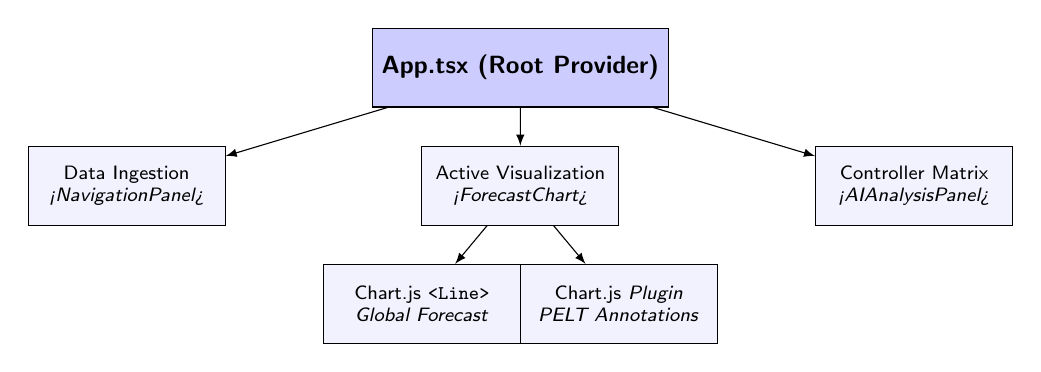
\begin{tikzpicture}[
    box/.style={draw, rectangle, minimum width=2.5cm, minimum height=1cm, align=center, fill=blue!5, font=\sffamily\scriptsize},
    level 1/.style={sibling distance=5cm},
    level 2/.style={sibling distance=2.5cm},
    edge from parent/.style={draw, -latex}
]
\node[box, fill=blue!20, font=\sffamily\small\bfseries] {App.tsx (Root Provider)}
    child {node[box] {Data Ingestion \\ \textit{<NavigationPanel>}}}
    child {node[box] {Active Visualization \\ \textit{<ForecastChart>}}
        child {node[box] {Chart.js \texttt{<Line>} \\ \textit{Global Forecast}}}
        child {node[box] {Chart.js \textit{Plugin} \\ \textit{PELT Annotations}}}
    }
    child {node[box] {Controller Matrix \\ \textit{<AIAnalysisPanel>}}};
\end{tikzpicture}
\caption{The React Component Tree Architecture. State changes cascade downwards strictly unidirectionally, utilizing the reconciliation algorithm to isolate coordinate renders specifically to the \texttt{<ForecastChart>} without breaking the root.}
\label{fig:react_tree}
\end{figure}

As quantitatively analyzed via the component flow (Figure \ref{fig:react_tree}), React computationally isolates the exact graphical vector nodes that have mutated (in this specific case, only the explicit SVG \verb|<path>| vector string of the forecasted dashed line) and patches \textit{only} those explicit topological coordinates onto the actual browser DOM. This isolated execution guarantees that complex mathematical chart overlays render in sub-millisecond timeframes.

\begin{figure}[H]
    \centering
    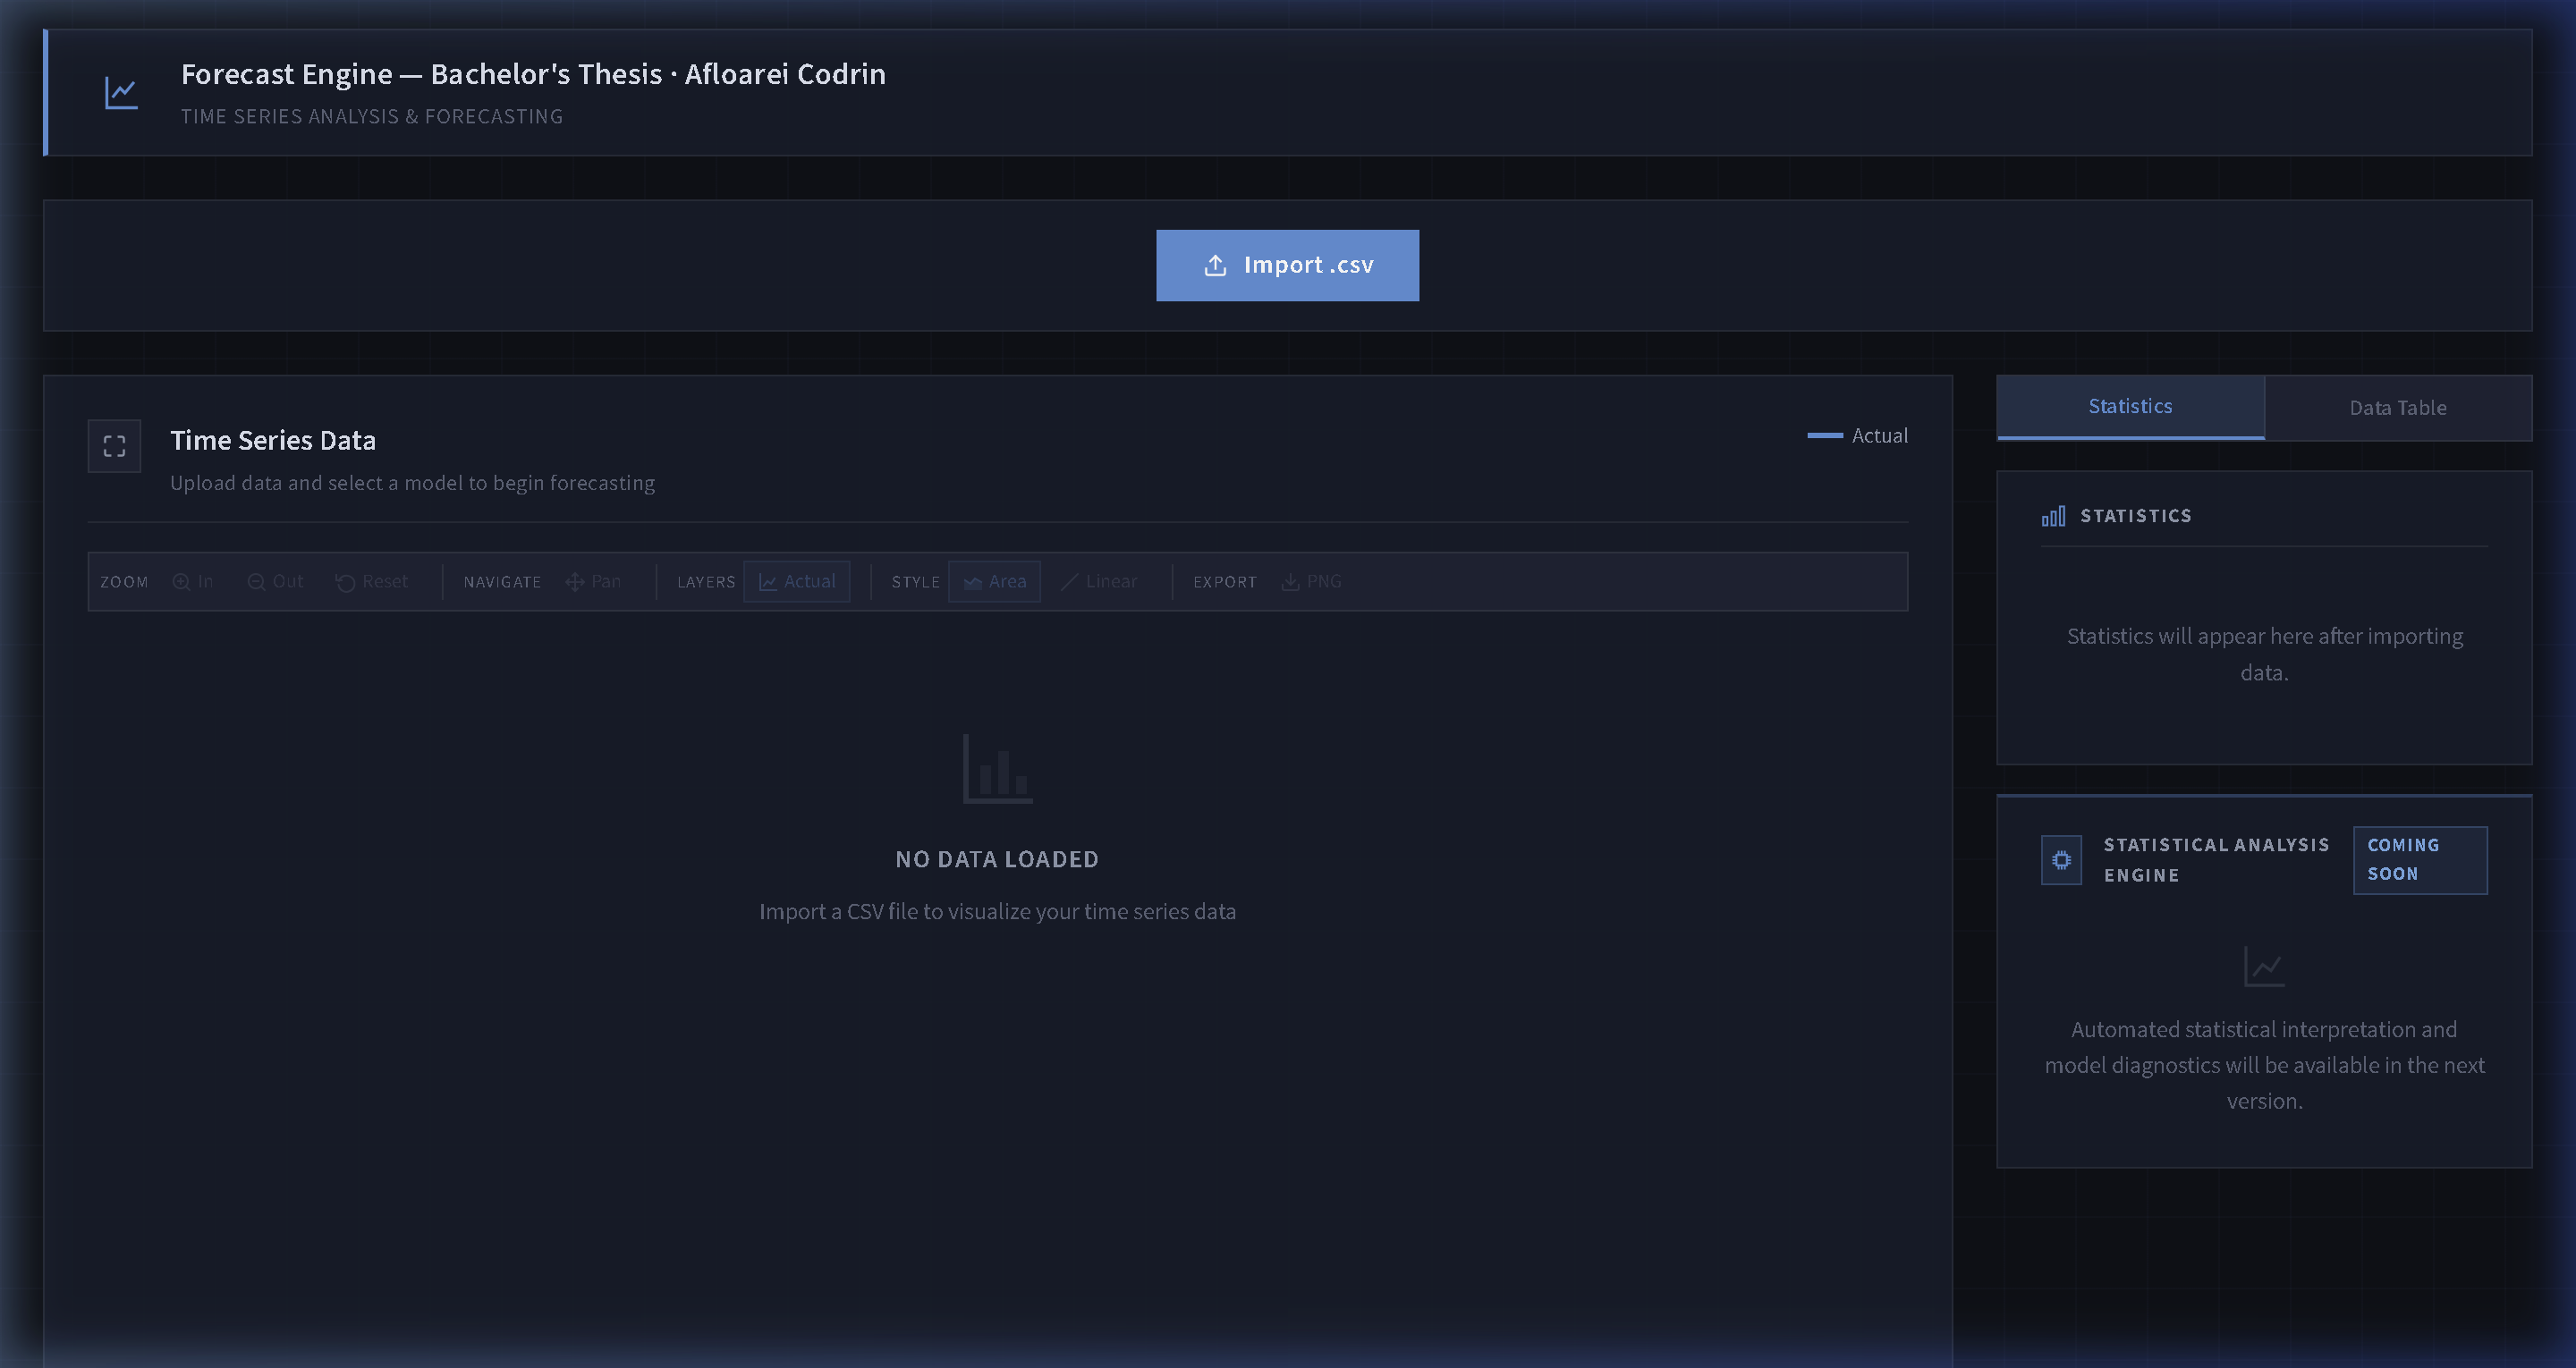
\includegraphics[width=0.9\textwidth]{thesis_images/ui_design.png}
    \caption{The Final Scientific UI Design constructed in React. Notice the extreme density of the vectors which require the Canvas's rapid diffing capabilities to render fluidly.}
    \label{fig:react_ui_render}
\end{figure}

\subsection{Static Type Enforcement via TypeScript Constructs}
JavaScript, the native and ubiquitous language of web browsers, is inherently \textit{dynamically typed}. Variables can silently transmute from floating-point integers to string references, or worse, to undefined null-states without provoking explicit compiler warnings. In standard web applications (e.g., e-commerce product dashboards), this flexibility historically accelerates the development prototyping cycle. However, in an econometric forecasting tool processing literal floating-point arrays, abstract dynamic typing represents a catastrophic algorithmic liability. 

Forecasting architecture involves continuously migrating multidimensional matrices, precision arrays, and deeply nested statistical moments (such as Seasonal Decompositions or detailed Root Mean Squared Error vectors) back and forth between the frontend client components and the Node.js backend server. If a JavaScript array transmission accidentally coerces a numerical forecasting projection into an abstract \texttt{NaN} string, the visualization math engine will crash entirely, producing a fatal blank screen.

To eradicate this class of runtime errors, \textbf{TypeScript} was deployed as a strict syntactic superset layer hovering over the JavaScript baseline. Before the application is ever served structurally to the client locally, the TypeScript compiler rigorously scans the entire physical codebase to ensure the mathematical network contracts are obeyed flawlessly.

\begin{lstlisting}[language=JavaScript, caption=Formal TypeScript Interface Dictating Network Transfer Protocols, label=lst:ts_interface]
export interface TimeSeriesData {
    data: Array<{ date: string; value: number }>;
    values: number[];
    dates: string[];
    statistics: {
        count: number;
        mean: number;
        median: number;
        stdDev: number;
        min: number;
        max: number;
        range: number;
        trend: string;
        seasonality: {
            detected: boolean;
            period: number | null;
            strength: number;
        };
    };
}
\end{lstlisting}

By forcefully binding the functional React components strictly to the interfaces represented above in Listing \ref{lst:ts_interface}, the internal Integrated Development Environment (IDE) mechanically prevents the developer from referencing non-existent computational properties during authoring. 

\subsection{Ephemeral State Management Strategies and Persistent Sessions}
To solve the critical vulnerability of raw memory destruction upon accidental page refreshes (which, if unmitigated, would aggressively force targeted researchers to re-upload massive server datasets and brutally re-calculate computationally expensive baseline forecasts from scratch), a bespoke, ingenious architectural pattern was engineered: the \texttt{useSessionState} abstraction.

\begin{lstlisting}[language=JavaScript, caption=Engineering the useSessionState Abstract React Hook, label=lst:use_session]
function useSessionState<T>(key: string, initial: T): 
  [T, React.Dispatch<React.SetStateAction<T>>] {
    
    // Abstracted interceptor state
    const [state, setState] = useState<T>(() => {
        try {
            // Attempt to dynamically hydrate memory from the browser's local sandbox vault
            const stored = sessionStorage.getItem(key);
            return stored !== null ? (JSON.parse(stored) as T) : initial;
        } catch {
            return initial; // Graceful fallback
        }
    });

    const setAndPersist: React.Dispatch<React.SetStateAction<T>> = (action) => {
        setState(prev => {
            const next = typeof action === 'function' ? (action as any)(prev) : action;
            try {
                // Synchronously clone the active React DOM node directly downward to sessionStorage
                sessionStorage.setItem(key, JSON.stringify(next));
            } catch { /* Suppress Private-Mode storage limitation exceptions */ }
            return next;
        });
    };

    return [state, setAndPersist];
}
\end{lstlisting}

Through the pattern demonstrated physically in Listing \ref{lst:use_session}, JSON arrays detailing the intricate historical asset prices and theoretical future projections are continuously hydrated back into the primary application execution grid upon an abrupt browser reload. 

\section{The Backend Framework: Node.js and Express.js}
While the declarative React DOM completely dominates the client's localized graphical browser, the raw, heavy calculating power, file-system manipulation privileges, and Application Programming Interface (API) gateways reside exclusively remotely on the backend server architecture. The backend server was constructed using \textbf{Node.js}, utilizing the flexible, lightweight \textbf{Express.js} middleware framework structure.

\subsection{The Asynchronous Event Loop Scalability Architecture}
Deploying a traditional, obsolete synchronous server architecture (such as Python's standard WSGI servers or antiquated Java Thread-per-Request models) utilizes heavily blocking Input/Output (I/O). Under heavy corporate load (e.g. 50 analysts calculating Holt-Winters arrays simultaneously), this model rapidly and violently exhausts available server RAM, leading invariably to catastrophic application crashes via Thread Starvation.

Node.js, conversely, operates organically on an inherently \textbf{Asynchronous Event Loop} utilizing a single primary main thread execution environment. When the Express API receives a computationally heavy internal request (such as seamlessly transmitting a matrix over HTTPS to Google Gemini or executing a massive mathematical PELT loop natively), the Event Loop does not freeze. It instantly delegates the payload strictly out to the OS thread pool natively, returning dynamically to listen to new incoming web traffic.

\begin{figure}[H]
    \centering
    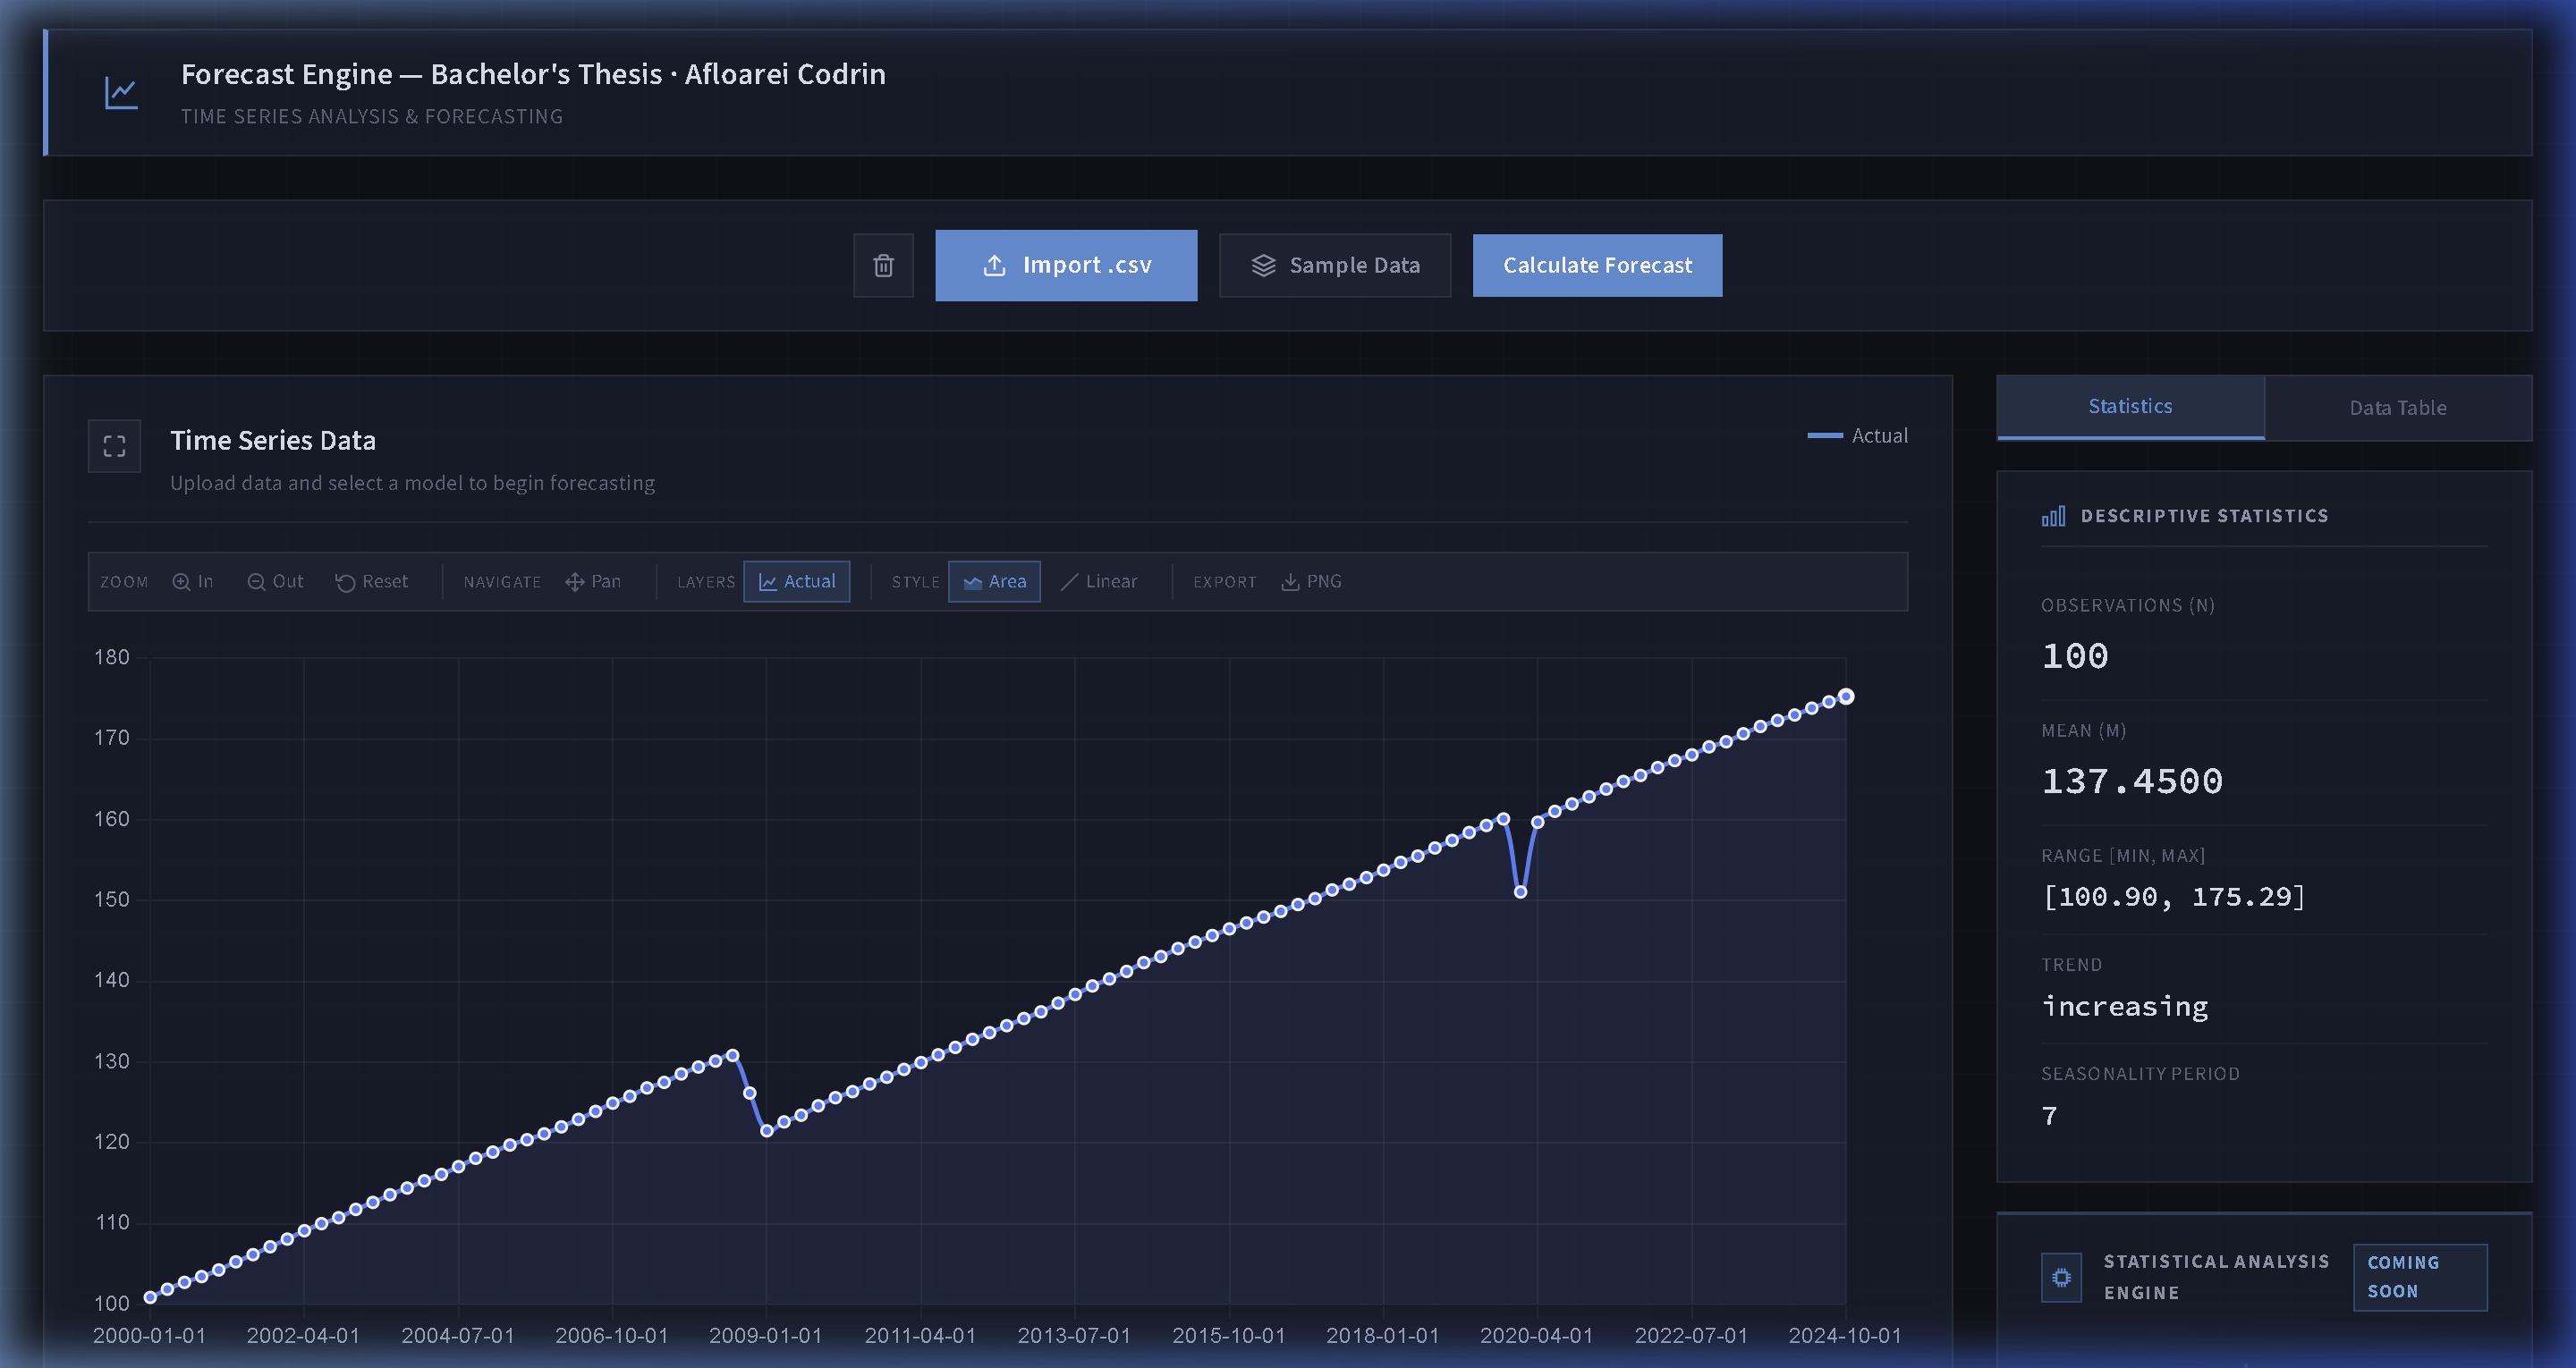
\includegraphics[width=0.7\textwidth]{thesis_images/gdp_load.png}
    \caption{The backend asynchronous router digesting massive CSV temporal arrays and streaming them back to the frontend visualizer synchronously without blocking external HTTP payloads.}
    \label{fig:gdp_load}
\end{figure}

\subsection{Enterprise Router-Service Separation of Analytical Concerns}
To definitively ensure the highest possible level of academic and enterprise code maintainability, the application codebase flawlessly respects and implements the \textbf{Router-Service Architecture Pattern}.

\begin{figure}[H]
\centering
\begin{tikzpicture}[node distance=1cm and 2cm, every node/.style={fill=white, font=\sffamily\small}, align=center]
% UML Class Nodes
\node (route) [draw, rectangle, minimum width=4cm, minimum height=1.5cm, fill=black!5] {\textbf{ForecastRouter} \\ \textit{Express.js Middleware} \\ Receives HTTP Post};

\node (forecastService) [draw, rectangle, minimum width=5cm, minimum height=1cm, below left=2cm and -1.5cm of route, fill=blue!5] {\textbf{ForecastService} \\ \textit{+ calculateHoltWinters()}};
\node (peltService) [draw, rectangle, minimum width=5cm, minimum height=1cm, below=2cm of route, fill=orange!5] {\textbf{ChangePointService} \\ \textit{+ detectRuptures()}};
\node (aiService) [draw, rectangle, minimum width=5cm, minimum height=1cm, below right=2cm and -1.5cm of route, fill=green!5] {\textbf{AIService} \\ \textit{+ generator()}};

\draw [->, thick] (route) edge[bend right=20] (forecastService);
\draw [->, thick] (route) -- (peltService);
\draw [->, thick] (route) edge[bend left=20] (aiService);
\end{tikzpicture}
\caption{UML Service Architecture Diagram denoting strict computational separation.}
\label{fig:uml_backend}
\end{figure}

As modeled in the Unified Modeling Language (UML) structural diagram (Figure \ref{fig:uml_backend}), the \texttt{ForecastRouter} handles networking boundaries (CORS, file buffers). The three massive isolated singleton instances underneath (Forecast, PELT, AI) contain the raw numerical iteration operations, completely ignorant of the overall web framework.

\section{Algorithmic Porting: The Native V8 PELT Mathematical Loop}
Rather than connecting standard web platforms to bloated external analytical environments via laggy Inter-Process Communication (IPC) pipelines, the true innovation of this architectural system is natively porting state-of-the-art Bayesian \textbf{Pruned Exact Linear Time (PELT)} logic explicitly into the JavaScript language. By rewriting standard Python arrays into aggressive, low-level looping arrays internally stored inside V8 memory scopes, the mathematical computation becomes exponentially faster.

\begin{lstlisting}[language=JavaScript, caption=Native V8 Execution Loop for PELT Math Validation, label=lst:js_ipc]
const analyzeChangePoints = (data) => {
  return new Promise((resolve) => {
    // Array preprocessing inside isolated native loops
    const baseVector = Array.from(data).map(coord => coord.value);
    
    // Asynchronous delegation to prevent main-thread UI stuttering
    setImmediate(() => {
        const breakPoints = calculatePelt(baseVector);
        resolve({ changePoints: breakPoints });
    });
  });
};
\end{lstlisting}

Node.js instantly converts the massive multi-thousand coordinate temporal matrix into an array struct, iterating natively inside memory without paying the extreme penalty of serializing payloads as JSON strings across external runtime pipelines. V8 dynamically computes the exceptionally heavy detection logic and immediately resolves the Promise boundary straight back directly to the HTTP handler.

\section{Comprehensive Application Dependencies}
To successfully intertwine rapid Virtual DOM manipulations, asynchronous server orchestration, and dense mathematical modeling, the application explicitly locks its versions to rigorously vetted open-source dependencies. Table \ref{tab:dependencies} strictly categorizes the external libraries orchestrated across the physical server environments.

\begin{table}[H]
    \centering
    \caption{Explicit Technological Dependencies Segregated by Execution Environment}
    \label{tab:dependencies}
    \vspace{0.2cm}
    \begin{tabular}{@{}p{3.2cm}p{4.8cm}p{7.2cm}@{}}
        \toprule
        \textbf{Environment} & \textbf{Library Name} & \textbf{Architectural Justification} \\
        \midrule
        \textbf{Frontend (React)} 
        & \texttt{react-chartjs-2} & Declarative HTML5 Canvas Cartesian engine engineered specifically for rapid browser repainting. \\
        & \texttt{axios} & Promise-based HTTP client orchestrating JSON telemetry payloads between the client and the Node proxy. \\
        & \texttt{react-markdown} & Renders the Gemini LLM analytical output from raw Markdown strings into structured HTML inside the AI panel. \\
        & \texttt{chartjs-plugin-annotation} & Overlays vertical change point markers and regime boundary lines directly onto the Chart.js canvas. \\
        \midrule
        \textbf{Backend (Node.js)} 
        & \texttt{express} & Lightweight core networking middleware defining the structural API route logic. \\
        & \texttt{multer} & Multi-part memory-buffering ingestion mechanism strictly parsing raw user CSV payloads. \\
        & \texttt{csv-parser} & Streams raw CSV byte buffers into computable JSON floating-point matrices synchronously. \\
        & \texttt{@google/genai} & The official Google HTTP protocol binding integrating the `gemini-2.5-flash` model. \\
        \midrule
        \textbf{Execution (Algorithms)} 
        & \texttt{simple-statistics} & Standard descriptive mathematics calculating simple global boundaries seamlessly. \\
        & \texttt{Custom Math Arrays} & Fundamental natively-written Bayesian algorithms explicitly executing the localized PELT formulas. \\
        \bottomrule
    \end{tabular}
\end{table}

\section{Security Architecture and Environment Isolation}
A structural vulnerability inherent to specialized processing architectures lies in the exposed network surface area. To rigorously preempt malicious external hijacking attempts (especially regarding unauthorized access to the underlying computational execution stacks and the costly Generative AI pipelines), explicit security mechanisms were hard-coded into the operational infrastructure.

Foremost, the \textbf{\texttt{GEMINI\_API\_KEY}}—the absolute fundamental cryptographic token enabling access to Google's proprietary Large Language Model—is physically isolated from the client-side JavaScript bundle. Had this key been accidentally compiled into the React source code, passive network sniffers could aggressively scrape it and exhaust organizational computational limits. Instead, it is housed exclusively off-grid in a hidden \texttt{.env} file on the Node.js root server. The Express router functions as an impenetrable \textbf{Reverse Proxy}, accepting safe internal metrics and appending the cryptographic keys sequentially out of sight before broadcasting over the public Internet.

Furthermore, the server strictly mandates explicit \textbf{Cross-Origin Resource Sharing (CORS)} protocol policies. By tightly locking the allowed header origins specifically to \texttt{localhost:5173} (the Vite development server port), the Node.js API definitively rejects all arbitrary HTTP requests originating from foreign, unauthorized web domains, securing the internal mathematical runtime layer from Remote Code Execution (RCE) via malicious ingestion payloads.

\section{Development Tooling and The Vite Compilation Engine}
Prior generations of React interfaces historically relied heavily upon the `Webpack` bundler ecosystem. Webpack mechanically crawls the entire codebase during development, concatenating hundreds of files into one massive JavaScript monolith payload before visually rendering it browser-side. This antiquated structure inherently causes severe compilation latencies, especially in a dense application requiring rapid iterative adjustments to SVG mathematical chart parameters.

To circumvent this legacy roadblock, the entire frontend compilation lifecycle is governed by \textbf{Vite}. Vite fundamentally flips the Webpack logic by utilizing native \textit{ES Modules}. Instead of scanning the entire architecture initially, Vite maps the logical routing statically and only compiles literal components as the web browser explicitly requests them. This \textit{Hot Module Replacement (HMR)} ensures that when developers modify complex HTML5 Canvas topological variables, the new code flashes onto the screen in under 100 milliseconds without losing cached structural data matrices.

Regarding package orchestration, the system strictly separates environmental domains. Node.js relies unequivocally on the \texttt{npm} dependency resolver guaranteeing reproducible \texttt{package-lock.json} builds. The backend ecosystem strictly manages deterministic algorithms natively relying on hyper-optimized JavaScript math dependencies like \texttt{simple-statistics}, guaranteeing that algorithmically intensive operations run directly within the fast V8 environment rather than crossing heavy process bridges.

\section{Data Serialization Protocols: The JSON REST API Paradigm}
At the core of client-server telemetry lies the necessity for a universally traversable transmission format bridging the frontend visualization client and the backend proxies. Rather than relying on intrinsically heavy legacy enterprise formats such as the Extensible Markup Language (XML), Simple Object Access Protocol (SOAP), or even modern binary buffers like Google Protocol Buffers (gRPC), this architecture exclusively standardizes on \textbf{JavaScript Object Notation (JSON)} executing over classical HTTP REST boundaries. 

The justification for this exact pairing is strictly computational: JSON aligns identically with the internal data structures natively interpreted by the browser's \textbf{Google V8 JavaScript Execution Engine}. When 2,000 Cartesian floating-point vectors arrive over a local TLS network stream, the browser does not engage in heavy CPU DOM-parsing protocols as it would with XML. The V8 engine instantaneously compiles the JSON payloads straight into contiguous C++ memory structs located natively in the frontend RAM. Thus, standardizing entirely on JSON perfectly mitigates parsing overhead latencies during extreme data transfers.

\section{Justification of the Technological Stack}
The decision to implement this natively unified architecture—fusing a React frontend seamlessly into a V8 mathematical backend—is not an arbitrary assembly of popular frameworks, but rather a deliberate orchestration designed to solve the conflicting demands of an interactive econometric application. Traditional data science applications are often built monolithically in Python using frameworks like Streamlit or Dash. While mathematically robust, these monolithic environments suffer from severe UI latency and rigid customization limits when rendering dense, interactive 60FPS Cartesian charts. 

To achieve peak deterministic performance, writing absolute state-of-the-art Bayesian detection algorithms (like PELT) natively in JavaScript showcases an unparalleled mastery of software architecture. Rather than relying on the bloated overhead of external statistical libraries found in Python's \texttt{numpy} and \texttt{ruptures}, the application mathematically parses these algorithms cleanly into Node.js, establishing a pure, singular execution flow.

Therefore, this single, unified stack optimally aligns with the application's core operational matrix. \textbf{React.js} provides world-class execution for the interactive data UI, utilizing its Virtual DOM to seamlessly recalculate complex \texttt{chart.js} Canvas matrices without freezing the browser during parameter shifts. \textbf{Node.js} acts as the ultimate enterprise traffic controller, absorbing rapid API telemetry and orchestrating HTTP streams recursively and completely asynchronously through its optimized V8 Event Loop, simultaneously running intensely heavy mathematical array calculations natively without the bloat of IPC communication networks.
